\documentclass[a4paper,11pt,openany]{article}
\usepackage[noconfigs,french]{babel}
\usepackage[utf8]{inputenc}
\usepackage[left=2cm,right=2cm,top=1.5cm,bottom=1.5cm]{geometry}
\usepackage{amsmath}
\usepackage{amssymb}
\usepackage{float}
\usepackage{appendix} 
\usepackage{graphicx}
\usepackage{hyperref}
\usepackage{listings}  
\usepackage{mathtools}

\title{Compression en diamants de maillages tetrahédriques}
\author{Gabriel Beauplet, Luca Castelli Aleardi}
\date{%
    Stage MPRI\\%
    \today
}

\begin{document}
\maketitle

\section{Abstract}
\section{Introduction}
\noindent
Un maillage représente un domaine géometrique en le discretisant en formes simples. Les maillages permettent de représenter des objets géométriques en 1, 2 ou 3D à des fins scientifiques ou industrielles par exemple. En 2D, les maillages representent des surfaces et sont constitués de polygones (triangles, carrés...) reliés deux à deux par une arête. En 3D, les maillages représentent des volumes à l'aide de polyèdres (tétraèdres, pyramides...) partageant une face commune. Les maillages sont très utilisés pour la visualisation de volume, calculs de solutions pour des équations aux dérivées partielles... Cependant, les maillages sont des structures complexes qui peuvent devenir très volumineuses et dont on essaye de réduire la taille.\\
La compression de données est omniprésente en informatique, avec des formats compressés génériques comme \textit{gzip} mais aussi dédiés comme \textit{mp3} pour les fichiers audios. Ce besoin de compresser les données est grandissant car de plus en plus de fichiers sont stockés à distance sur des serveurs et la moindre économie de stockage a d'importantes répercussions. Néanmoins, sous certains formats compressés, les données originales deviennent inutilisables (ex : \textit{rar}). Cela pose problème quand l'on souhaite accéder aux données  sans passer par l'étape de décompression.\\
Une structure de données est une manière d'organiser les données pour faciliter leur traitement. Les listes, arbres et graphes sont des exemples de structures de données. Leur but n'est pas de limiter l'usage mémoire mais seulement de faciliter l'utilisation des données. Ainsi, pour certains formats volumineux, des structures de données compactes ont été inventées. Ce sont des structures de données compressées, des structures de données dont l'utilisation de la mémoire est limitée.\\
Si l'on revient aux maillages, les algorithmes de compression limitent au maximum l'usage mémoire du maillage et il devient inutilisable sous forme compressé tandis que la structure de données pré-traite le maillage en réduisant l'usage mémoire mais celui-ci reste utilisable. Les maillages en deux dimensions sont majoritairement utilisés car ils sont plus léger, et permettent de représenter implicitement des volumes (la frontière). Par conséquent, de nombreuses structures de données compactes ont été créees afin de faciliter leur utilisation. Les maillages 3D étant beaucoup moins utilisés pour l'instant, peu de structure de données compactes leur sont dévolues. Néanmoins, leur utilisation croissante incite à procéder de même. La suite de ce rapport sera principalement consacrée aux structures de données compactes pour maillages 3D tétraèdriques.\\\\
De manière générale, un structure de données pour maillage stocke trois types d'informations :
\begin{itemize}
\item La géometrie, c'est à dire les positions des sommets
\item La connectivité, les relations d'adjacence entre les tétraèdres
\item Des attributs (par sommet, par arête, par face, par tétraèdre)
\end{itemize}
La structure de données doit supporter des requêtes simples :
\begin{itemize}
\item Quels sont les sommets de la ième face ?
\item Quel est le degré du ième sommet ?
\item Quelles sont les tétraèdres adjacents au ième tétraèdre ?
\item ...
\end{itemize}
Par ailleurs, suivant l'utilisation ciblée, la structure de données devra être en mesure de satisfaire des opérations de modification :
\begin{itemize}
\item Ajouter/Enlever un sommet
\item Ajouter/Enlever/Séparer un tetra\\
\end{itemize}
%Finalement, le fonctionnement de la structure de donnée doit être simple pour permettre sa ré-implémentation.\\
On évalue une telle structure de données en analysant le temps nécessaire à sa construction, à l'exécution d'une requête, à une opération de modification et surtout en observant la quantité de stockage nécessaire pour l'utiliser.\\\\
\textbf{Contributions}. Dans ce rapport, nous présentons une structure de données permettant de représenter la connectivité d'un maillage tetrahedrique en utilisant en moyenne 2.4 références par tétraèdre. Notre structure s'appelle \textit{Tétraèdres en diamant}. Elle permet par ailleurs l'accès au ième sommet, au ième tétrahèdre et à l'étoile d'un sommet en temps constant. Son implémentation est simple et l'utilisation d'un tableau d'entiers afin de représenter les références permet une interopérabilité entre les languages de programmation.\\
Nous allons d'abord définir les principaux termes utilisés et rapeller les algorithmes de compression et structures de données déjà développés en deux et trois dimensions. Puis nous présenterons le fonctionnement, les avantages et inconvénients de notre structure de données. Par ailleurs, nous comparerons notre structure de données avec d'autres structures en terme de stockage mémoire ou de coût de calcul.

\subsection{Définitions}
\noindent
\textbf{Simplexe}. Un simplex $\sigma^p$ de dimension $p$ est l'enveloppe convexe de $p+1$ points $\{v_0,v_1,...v_p\}$, où $v_i\, \in R^n$ et les vecteurs $v_1-v_0,v_2-v_0...$ sont linéairement indépendants. Les simplexes de dimensions 0, 1, 2 et 3 sont respectivement les sommets, arêtes, triangles et tétraèdres.\\\\
\textbf{Complexe simplicial}. Un complexe simplicial est un ensemble K de simplexes d'un espace affine tel que toutes les faces de chaque simplexe de K appartiennent aussi à K et si deux simplexes $\sigma$ et $\tau$ de K sont adjacents alors $\sigma \cap \tau \neq \emptyset$.\\\\
%Les points $v_0,v_1,...v_p$ sont appelés les sommets de $\sigma$. 
%Une face est l'enveloppe convexe d'une partie des sommets (pas tout). Si un simplex $\sigma$ est la face d'un simplexe $\tau$, alors $\tau$ est dit incident et $\tau$ limite $\sigma$. La frontière d'un p-simplexe $\sigma$ $\partial \sigma$ est la collection de toutes ses faces.\\\\
%\textbf{Etoile}. L'étoile ouverte d'un simplexe $\sigma \in K$ noté étoile($\sigma$,$K$) est l'union de tous les simplexes de l'étoile avec ses faces.\\\\
\textbf{Variété}. Une variété topologique (manifold en anglais) M de dimension n est un espace topologique connexe séparé localement homéomorphe à un ouvert de $\mathbb{R}^n$. C'est à dire que chaque point de M admet un voisinnage homéomorphe à un ouvert de $\mathbb{R}^n$.\\\\
\textbf{Variété à bord}. Une variété à bord est un sous-espace topologique dont les points admettent un voisinage homéomorphe à $\mathbb{R}^n$ (les points intérieurs) ou un voisinage homéomorphe à $\mathbb{R}^{n-1}  x \mathbb{R}^+$ (les points bordants). L'ensemble des points bordants constitue le bord de la variété.\\\\
\textbf{Frontière}. Les (k-1)-simplexes d'une k-variété $M$ qui sont incidents à seulement un k-simplexe sont les simplexes frontières. L'ensemble des simplexes frontières est dénoté $\partial M$.\\\\
%Une k-variété est orientable s'il est possible de choisir une orientation cohérente pour tout ses simplexes. Une orientation est cohérente si deux k-faces adjacentes induisent deux orientations opposées sur leur (k-1)-face.
%Un complexe simplicial  $M$ est une k-variété si l'étoile ouverte d'un sommet dans $M$ est homeomorphique à $R^k$ ou à $R^{k-1}XR_+$. En particulier, si $M$ est une variété alors tout (k-1)-simplex dans $M$ est la frontière de un ou deux k-simplexe.\\
\textbf{Maillage}. Un maillage est un complexe simplicial representant un objet géométrique. Il à la même dimension que l'objet qu'il représente. Ainsi, pour tout objet en 1, 2 ou 3D, les maillages respectifs seront en dimensions 1, 2 ou 3. Dans un maillage de dimension d, les simplexes de dimensions (d-1) sont appelées des facettes. Ainsi, les facettes d'un tétraèdre sont ses faces, les facettes d'une face sont ses arêtes et les facettes d'une arête sont ses sommets.\\\\
\textbf{Le degré}. Le degré d'un k-simplexe est le nombre de (k+1)-simplexes adjacents. Ainsi le degré d'un sommet est le nombre d'arêtes adjacentes et le degré d'une arête est le nombre de faces adjacentes.\\\\
\textbf{Etoile}. L'étoile d'un sommet est l'ensemble des k-simplexes adjacents à un sommet. C'est l'ensemble des triangles (resp. tétraèdres) adjacents à un sommet dans le cas surfacique (resp. volumique).\\\\
%Nous traitons dans ce rapport de maillages tetrahedriques dans un espace Euclidien à 3 dimensions. Deux tetrahedres sont dit adjacents s'ils partagent une face. On dénote par V l'ensemble des sommets, E l'ensemble des arêtes, F l'ensemble des faces et T l'ensemble des tetrahedres du maillage.\\
%En utilisant l'équation d'Euler, on a la relation suivante : 
%\begin{equation}
%|V|-|E|+|F|-|T|=\chi
%\end{equation}

\subsection{Combinatoire}
\noindent
En mathématique et en optimisation combinatoire, la caracéristique d'Euler $\chi$ est un invariant topologique décrivant la forme d'un objet géométrique.
\begin{equation}
\chi = \sum_{i=0} (-1)^i \, |dim(H_i)| = 2-2g
\end{equation}
\begin{itemize}
\item $H_i$ est l'ensemble des faces de dimension $i$
\item $g$ est le genre (le nombre de trou de l'objet étudié)\\ 
\end{itemize}
Ainsi, pour un polytope de dimension 4, la formule d'Euler devient :\\
\begin{equation}
\chi = |V|-|E|+|F|-|T|
\end{equation}
\begin{itemize}
\item $V$ est l'ensemble des sommets
\item $E$ est l'ensemble des arêtes
\item $F$ est l'ensemble des faces (ie. polygone)
\item $T$ est l'ensemble des tétraèdres\\
\end{itemize}
Sachant que chaque face qui n'est pas sur les bords du volume est partagée par deux tétraèdres, alors :\\
\begin{equation}
|F|\simeq 2|T|
\end{equation}
Ainsi :
\begin{equation}
\chi \simeq |V|-|E|+|T|
\end{equation}
Il y a donc autant d'arêtes que de tétraèdres et sommets réunis.

\section{Etat de l'art}
\noindent
Les maillages sont la pluspart du temps stockés sous forme indexés. Dans un premiers temps, on énumère pour chaque sommet ses coordonnées géométriques. Puis pour chaque face (resp. tétraèdre), les indices de ses 3 (resp. 4) sommets. D'autres attributs peuvent être stockés (normales, couleurs...) mais nous n'en discuterons pas ici. Les formats indexés ne sont pas les formats les plus concis pour sauvegarder des maillages. En effet, la connectivité occupe une place très importante. Tandis que dans les maillages 2D, le degré moyen des sommets est de 6, il est de 22 dans les maillages tétraèdriques. Par conséquent, dans ce type de format, un sommet apparaitra dans 22 tetras différents.\\
%La compression de maillages peut être séparer en 3 catégories : simplification polyhedrale, compression de positions, compression des informations de connectivités.\\\\
%\textbf{La simplification polyhedrale} consiste à simplifier le maillages en réduisant le nombre de sommets et en modifiant leurs positions afin que le nouveaux maillages reste aussi proche que possible de l'ancien. Ce sont des compression de maillages avec perte et ne sont donc pas adaptés aux usages nécessitant le maillage exact.\\\\
%\textbf{Compression des positions}\\\\
%\textbf{Compression de la connectivite}. La compression des informations de connectivité permet de réduire la redondance d'informations d'adjacence entre les k-simplexe d'un k-objet.\\\\
%En effet, comme dit dans la première partie, la structure de données doit être capable de répondre à des requetes simples (ex: donner les tetras adjacents à un tetra). Sans compression, cela signifie que chaque tetra doit stocker 4 références vers ses 4 tetras voisins. De plus, si l'on veut connaître les sommets composants un tetra, il est nécessaire de sauvegarder 4 references vers les 4 sommets composant le tetra. Ainsi, nous avons 8 références par tetra. Par conséquent, dans un maillage contenant 10000 tetras et en utilisant des références sur 32 bits, nous utiliserions 10000*8*32=2mo de références.
%On distingue les algorithmes de compression de maillages des structure de données pour maillages. Les premiers tentent de limiter au maximum l'usage mémoire du maillage en compressant le maillage. Le maillage devient inutilisable sous forme compressé, il est nécessaire de le décompresser pour l'utiliser à nouveau. En revanche, la structure de données pré-traite le maillage mais le maillage reste utilisable sous forme compressé.\\
La mesure utilisée pour évaluer la qualité d'une compression est le nombre de bits par sommets (bits per vertex ou bpv). Tandis que la mesure utilisée pour évaluer la qualité d'une structure de données compacte est le nombre de références par triangle (resp. tétraèdre) rpt pour les maillages surfaciques (resp. volumiques).\\
On peut compresser un maillage en le simplifiant (supprimer des sommets...), en encodant la géométrie et/ou la connectivité du maillage. Nous ne nous intéresserons dans cette partie qu'à la compression de la connectivité puisque c'est la plus gourmande en mémoire. Par ailleurs, nous détaillerons d'abord le travail effectué en 2D puis en 3D. Bien que notre travail soit uniquement centré sur les maillages 3D, l'essentiel des travaux effectués jusqu'à présent est en 2D.
\subsection{Maillages 2D}
\subsubsection{Compression}
\noindent
\textbf{Bande de triangle}. Les bandes de triangles ("triangles strips") et les eventails de triangles ("triangle fans") sont des représentations utilisées pour transférer les maillages de la mémoire centrale du PC vers la mémoire du GPU. Une bande de triangle est une séquence de sommet où chaque nouveau sommet défini un triangle avec les deux précedent sommets. En ce qui concerne les bande de triangles, le but est de trouver de très longues bandes. Si les bande de triangles sont suffisament longue alors, cette representation permet de passer de 3N references aux sommets à N+2. L'algorithme de Deering utilise ces bandes de triangles et utilise entre 3.3 et 9.8 bpv \cite{triangle_strips}.\\\\
\textbf{Traversée de triangles}. La Cut border Machine \cite{cut_border_machine_2d} est un algorithme de Gumhold qui encode la conectivité en parcourant le graphe en largeur. L'algorithme étend la frontière défini par un triangle initial en travesant itérativement des triangles adjacents. Sept symboles sont utilisés pour préciser si la frontière a été étendu en insérant un nouveau sommets, si la frontière a été séparée ou si deux frontière se sont jointes. Le schéma peut compresser des variétés avec 4 bpv. En revanche, ce résultat est seulement valide pour des maillages réguliers. En effet, quand une jointure est effectuée, un décallage doit etre fait pour désigner les sommets concernés. Par conséquent, il n'y a pas de borne supérieure garantie pour la compression avec cet algorithme.\\
L'algorithme EdgeBreaker de Rossignac \cite{edgebreaker} traverse lui aussi le graphe d'un triangle adjacent à un autre et enregistre la connectivité d'un maillage en produisant les sympboles C,L,R,E,S. Cependant, il garantit un cout de 4bpv.\\\\
\begin{figure}[H]
\begin{center}
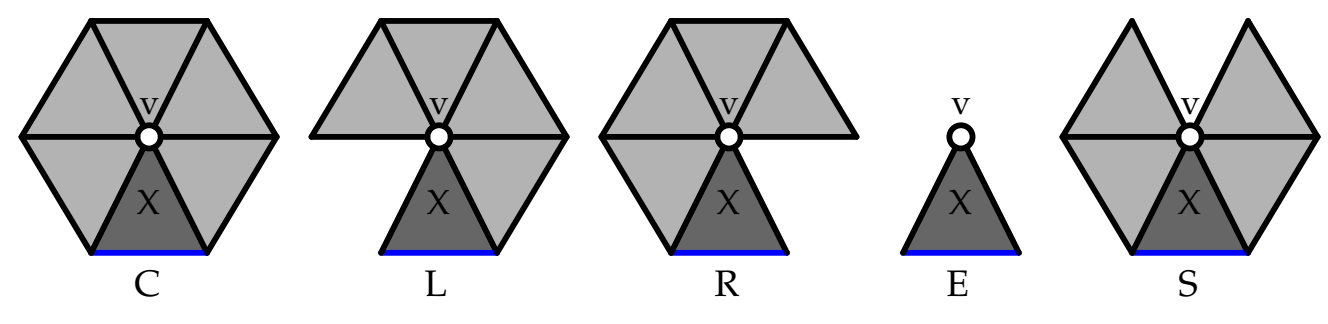
\includegraphics[scale=0.2]{Images/edgebreaker}
\caption{Les cinq configurations dans l'algorithme Edgebreaker. v est le sommet central de la configuration et X est le triangle cible}
\label{fig:edgebreaker}
\end{center}
\end{figure}
\noindent
\textbf{Codage de la Valence}. Une manière de décrire la connectivités de sommets est à travers leurs valence. Le premier travail sur la valence des sommets est le travail de Touma et Gotsman \cite{valence_encoding}. Le principe est de considérer la frontière d'un triangle initial et de l'étendre en ajoutant itérativement de nouveaux sommets. La connectivité est encodée en utilisant la valence des nouveaux sommets (concentrée autour de 6). Ainsi, La liste de valence des sommets peut être efficacement compressée par un encodeur d'entropie (2.3 bpv). C'est toujours aujourd'hui l'une des méthodes les plus efficace.
%Un maillage surfacique contient environ deux fois moins de sommets que de triangles. Par conséquent un algorithme qui se concentre sur l'insertion de nouveaux sommets (et qui génère un symbole par sommet) sera plus efficace qu'une traversée des faces du graphe. Ainsi, si l'entropie par symbole n'est pas deux fois plus large alors l'algorithme apportera de meilleurs taux de compression.\\
\subsubsection{Structure de données compacte}
\noindent
Plusieurs structures de données permettent une utilisation très facile des maillages et se focalisent sur l'utilisation des arêtes du graphe. C'est le cas d'Half-Edge, Winged-Edge et Quad-Edge qui stockent respectivement $18n$ et 9$n_t$ références. Elles permettent facilement de naviguer dans le maillage et opèrent des requêtes d'adjacence en temps constant. Cependant, elles occupent trop de place pour être considérées comme compactes.\\
La Corner Table (CT) est à la base de plusieurs structures de données. Elle utilise deux listes V et O de $3|F|$ entiers chacune. La table V stocke les incidence triangle/sommet tel que les 3 sommets bordant un triangle t sont consécutifs (V[3t],V[3t+1],V[3t+2]) et sont listés dans un ordre consistent avec le maillage. Ainsi, V[c] représente un coin c associé avec une face f et un sommet. La table O stocke la référence entière du coin oposé. Le coin opposé o(c) au coin c est un coin dans un triangle adjacent qui partage la même arête opposée.
\begin{figure}[H]
\begin{center}
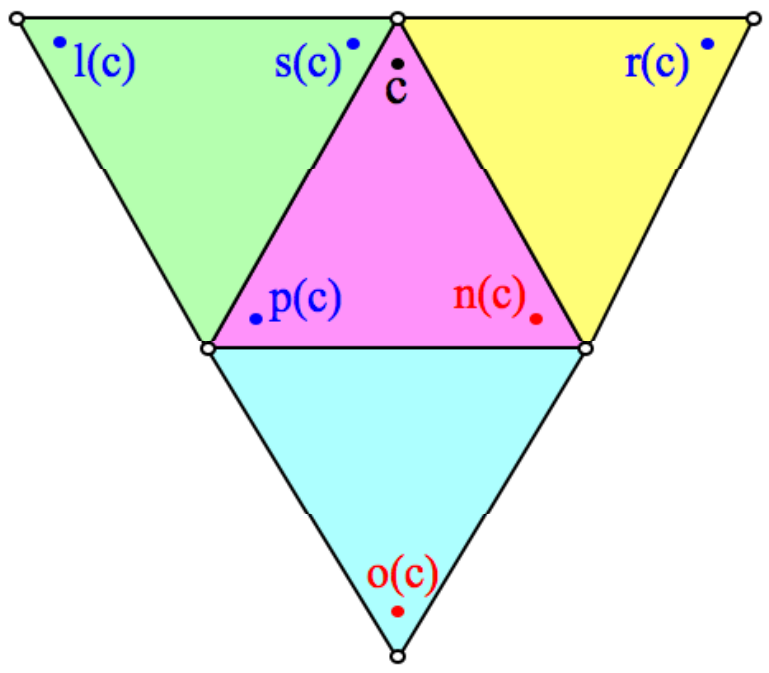
\includegraphics[scale=0.2]{Images/corner_table}
\caption{Les opérateurs utilisant les coins pour un maillage triangulaire}
\label{fig:corner_table}
\end{center}
\end{figure}
\noindent
\textbf{VOT}. La structure de données VOT (Vertex Opposite Table) est la première structure de données à utiliser cette "Corner Table". Elle permet une répresentation simple et efficace des maillages avec 6 références par triangle (3 références pour les sommets dans la table V et 3 référence pour les coins dans la table O).\\
\textbf{SOT}. SOT, développée par Rossignac \cite{SOT} est une amélioration de VOT où la table O est réordonnée et la table V supprimée. Néanmoins, l'accès au coin d'un sommet et à l'étoile d'un sommet sont toujours en temps constant. Cette dernière structure de données utilise 3 rpt en moyenne.
%\subsubsection{Enumération de triangulations planaires}
%La connectivité d'un maillage peut etre vu comme un graphe. Pour les maillages surfaciques, les sommets sont des noeuds connectés via les arêtes du graphes pour former des faces.
%%Cette analogie entre maillage et graphe explique pourquoi certains résultats très connu de la théorie des graphes peuvent etre appliqués pour la compression de la connectivité des maillages.
%Tutte a d'abord proposé une formule pour énumérer les triangulations planaires. Cette première énumeration permet de calculer ce que l'on appelle l'entropie de Tutte. Cette entropie vaut environ 3.25 bpv (bits per vertex). C'est une borne supérieure pour l'entropie de la connectivité de n'importe quel maillage surfacique.
%L'affichage de maillages important demande beaucoup de ressources en calcul. Les GPU sont fait pour réaliser ces opérations d'affichage rapidement en parallele. Par conséquent, les solutions permettant de transeferer le maillage de la mémoire centrale du PC vers la mémoire du GPU sont particulierement intéressante car les trasnfere de données demande beaucoup de cycles CPU. Ainsi, une bonne méthode de transfert de données peut senseiblement réduire le temps d'affichage.


%L'un des premiers travaux de compression est le "generalized triangle mesh format" de Deering qui inclut une généralisation des bandes de triangles. Deering a remarqué que les sommets intérieurs sont encodés deux fois. Par conséquent, il proposa de les mettre dans une file de 16 positions et de referencer les sommets par leur location dans cette file si besoin. Cette file permet de réduire le coût de la réutilisation de sommets. Neanmoins, en moyenne les sommets sont toujours utilisés deux fois, ce qui n'est pas effiface). Les résultats expérimentaux montrent que l'algorithme de Deering donne des taux de compression de 3.3 à 9.8 bpv.


\subsection{Maillages 3D}
\subsubsection{Compression}
\noindent
\textbf{Grow\&Fold}. L'algorithme Grow\&Fold \cite{grow_and_fold} combine les idées de l'algorithme Topological Surgery \cite{topological_surgery} de Taubin et EdgeBreaker \cite{edgebreaker} de Rossignac. Il construit un arbre couvrant de tétraèdre et un folding string. L'arbre couvrant début à une face arbitraire et grandit en ajoutant des tétraèdres aux faces externes de l'actuel arbre couvrant. Pour chaque ajout de tétraèdre, 3 bits encodes si d'autres tétraèdres seront attchés aux 3 faces extérieures de ce tétraèdre. Le folding string contient pour chaque triangle externe de l'arbre couvrant un code sur 2 bits permettant de retrouver les relations d'incidences absentes de l'arbre couvrant. L'abre couvrant contient $|T|$ tétraèdres et il y a $2|T|$ faces externes. Par conséquent, l'usage mémoire est de 7 bpt.\\
%L'algorithme "Grow and Fold" de Rossignac encode les tétraèdres en utilisant un peu plus de 7 bpt. Leur algorithme construit un arbre couvrant dans le graphe dual en partant d'une face arbitraire. L'arbre est encodé en utilisant 3 bpt par face indiquant pour chaque face si l'arbre couvrant va continuer de grandir. La frontière de l'arbre couvrant, un maillage surfacique a un "folding string" représenté avec 4 bpt et permettant de retrouver les relations d'incidences absentes de l'arbre couvrant en utilisant les opérations "folding" et "gluing".
\textbf{Cut Border Machine}. La Cut Border Machine pour les maillages volumiques \cite{cut_border_machine_2d} est directement inspirée de celle pour les maillages surfaciques de Gumhold \cite{cut_border_machine_3d}. L'algorithme étend la frontière défini par une face initiale en traversant des tétraèdres adjacents. Dix symboles sont utilisés pour décrire l'entourage de la frontière lors de l'ajout d'un nouveau sommet pour la construction d'un tétraèdre. Leur algorithme permet de compresser les maillages tétraèdriques en utilisant 2.4 bpt et s'adapte aux non-variétés.
 
\subsubsection{Structure de données compacte}
\noindent
\textbf{VOT}. La Corner Table a été adapté par Rossignac aux maillages tétraèdriques (VOT). Elle demande 8 rpt (4 pour les sommets et 4 pour les coins opposés). Un index dans ces listes identifie un coin particulier à un tétraèdre. Ainsi, les tables O et V ont toutes les deux $4|T|$ entrées. Les coins de chaque tetrahèdre sont consécutifs dans les deux listes (les quatres coins du ième tetra sont stockées aux entrées  4i+j, where j = 0,1,2,3) et sont listés dans un ordre consistent avec l'orientation du tétrahèdre (les sommets des coins j=1,2,3 apparaissent dans le sens inverse des aiguilles d'une montre depuis le sommet du coin 0).\\
\textbf{Bande de Triangles}. Weiler et al. \cite{triangle_strips_weiler} encode les tétrahèdres en bandes. L'inclusion d'une petite quantité d'informations d'adjacence leur permet d'acceder aux faces voisines en temps constant. Leur algorithme stocke en moyenne 5.1 rpt.\\
\textbf{SOT}. La dernière structure de données développée est SOT \cite{SOT} par Rossignac. Elle améliore sa première structure de données VOT en triant la table O et en supprimant la table V. La structure de données utilise 4 références et 9 bits par tétraèdre en moyenne et permet l'accès à l'étoile d'un sommet en temps constant.

%\textbf{Half-face}.  The Compact Half Face (CHF)
%proposed by Lage et al. extends CT to tetrahedral meshes, storing
%8 references per tetrahedron (4 in the V table and 4 in the O
%table)
%.  We call it the Vertex Opposite Table (VOT) and propose a
%sorted variation, SVOT, which does not require any additional
%storage and yet provides, for each vertex, a reference to an
%incident corner from which an incident tetrahedron may be
%recovered and the star of the vertex may be traversed at a constant
%cost per visited element. We use a set of powerful wedge-based
%operators for querying and traversing the mesh. Finally, inspired
%by tetrahedral mesh encoding techniques used by Weiler et al. and
%by Szymczak and Rossignac, we propose our Sorted O Table
%(SOT) variation, which eliminates the V table completely and
%hence reduces storage requirements by 50% to only 4 references
%and 9 bits per tetrahedron, while preserving the vertex-toincident-corner references and supporting our wedge operators
%with a linear average cost. 

%
%Their “Grow&Fold” technique codes tetrahedral connectivity using
%slightly more than 7 bits per tetrahedron (bpt). The encoding pro-
%cess builds a tetrahedral spanning tree rooted in an arbitrary bound-
%ary triangle. This tree is encoded with 3 bpt that indicate for each
%face whether the spanning tree will continue growing. The bound-
%ary of the tetrahedron spanning tree, a triangular surface mesh, has
%an associated “folding string” that is represented with 4 bpt. This
%string describes how to “fold” and occasionally “glue” the boundary
%triangles of the spanning tree to reconstruct the original connectiv-
%ity. The indices associated with the occasional “glue” operations
%lift the total bit rate slightly above 7 bpt
%
%Gumhold et al. have extended their connectivity coder for trian-
%gular surface meshes [5] to tetrahedral volume meshes [4]. Their
%algorithm performs a region growing process that maintains a “cut-
%border,” a (possibly non-manifold) triangle surface mesh, that sepa-
%rates processed tetrahedra from unprocessed ones. Each iteration of
%the algorithm processes a triangle on the cut-border, either declar-
%ing it a “border” face or including its adjacent tetrahedron inside
%the cut-border. The latter operation specifies the fourth vertex of
%the tetrahedron. If this is not a “new vertex” it is a vertex from the
%cut-border, which is specified with a “connect” operation using an
%indexing scheme that is based on a local breadth-first traversal. Be-
%cause of the order in which cut-border triangles are processed, this
%fourth vertex is often close to the processed triangle, and thus has
%a small local index. The bit rates they achieve for connectivity are
%around 2 bpt, a result that has not been challenged since.


\section{Diamond Compression}
\subsection{Le principe}
Dans citation, ils regroupaient les tetrahedres deux à deux afin d'économiser une reference d'un tetrahedre à l'autre. L'idée ici est de regrouper les tetrahedres partageant une même arrete. On appelle un tel regroupement un diamant.
Au sein d'un diamant, les tetrahedres sont ordonnés. On peut donc oublier les références de voisinage entre deux tetrahedres du même diamant (le tetrahedre 7 est connecté au tetra 6 et 8).
Ainsi, pour chaque tetrahedre d'un diamant, il est connecté à deux tetras du même diamant (un avant et un après). Ainsi, seul, pour chaque tetra du diamant, seul deux references sont necessaires afin de savoir quels sont les deux tetras adjacents n'appartenant pas au diamant.
Ainsi, dans le cas parfait, si tous les tetras étaient regroupés en diamants, alors la structure de données n'utiliserait que deux references par tetra.
\subsection{Appariement tetras en diamants}
La première étape est de regrouper les tetras en diamants. C'est à dire, trouver un ensemble maximum d'arêtes tel qu'aucune arête n'appartienne au même tetra.
Les tetras n'ayant aucune arête dans cet ensemble seront appelés des tetras isolés.
Pour trouver cet ensemble d'arêtes, nous avons essayés plusieurs algorithmes.

mettre image du cas de figure que l'on ne veut pas (deux aretes qui appartiennent au même tetra)

\subsubsection{Choisir l'arête la plus pentu pour chaque sommet}
La première méthode consiste à prendre pour chaque sommet, l'arête étant la plus pentu. Néanmoins, cette méthode a deux incovénients majeurs : deux arêtes peuvent être choisi et appartenir au même tetra, elle utilise la géometrie du domaine (et donc peut sembler moins générique).

\subsubsection{BFS}
La seconde approche consiste à parcourir le maillage en largeur. On choisit un tetrahedre au début de l'algorithme puis on regarde pour chacune de ses arêtes si elle forme un diamant et si aucun des tetrahedres n'est deja dans un diamant. Si c'est le cas, on ajoute ce nouveau diamant, sinon, on ajoute les tetras adjacents à la file.
On continue cet algorithme tant que tous les tetras n'ont pas été parcouru.

\paragraph{Choix du Tetrahedre de départ}
Le choix du tetrahedre de départ n'affecte que très légerement la qualité de l'algorithme.

mettre image de l'incidence du tetra de début

\paragraph{BFS ou DFS}
DFS semble donner des résultats moins bon que BFS.

\paragraph{Inconvénient}

En utilisant un outil de visualisation de maillages 3D réalisé par Luca Castelli, on s'appercoit que les tetra isolés sont essentiellement sur les bords du domaine. Par conséquent, nous avons essayé de constituer les diamants d'abord sur les bords mais sans reussite.
 
\subsection{Algorithme randomisé}
L'idée est d'utiliser un algorithme randomisé afin de selectionner les arêtes centrales des diamants. On assigne donc un 0 ou 1 à chaque arête suivant si la solution la contient ou non. Puis on calcule la qualité de la solution en utilisant une fonction de fitness qui assigne +1 pour chaque tetrahedre dans un diamant et -1 si deux arêtes appartiennent au même tetrahedre.

L'avantage de cet algorithme est qu'il permet de trouver des solutions de meilleures qualités. Cependant, son execution est plus longue et ne garantie aucune propriété sur la solution finale.

\subsection{BFS+algorithme randomisé}
La solution finale est donc un mélange de BFS et d'algorithme randomisé. BFS offre une solution convenable en un temps très court. Néanmoins, sa solution peut etre améliorer avec un algorithme randomisé.


Nous avons donc sélectionné un ensemble d'arêtes representant les diamants. Tous les tetrahedres ne possedant pas une de ces aretes sont dit isolés.
\subsection{Choisir l'ancre}
Il est necessaire d'acceder au ième sommet facilement. Afin de ne pas ajouter de references, on associe à chaque edge central d'un diamant un sommet. Ainsi, pour chaque diamant, il y a un sommet affecté à celui-ci.
Si un sommet n'a aucun diamant voisin (que des tetras isolés) alors, on associe le sommet à un des tetras isolés.
Si un sommet n'a aucun diamant de libre dans son voisinnage alors, on explose un diamant (on supprime le diamant, et on fait comme si il n'y avait que des tetras isolés) et on affecte le sommet à un de ces tetras isolés.

montrer la figure représentant tous les edges centraux

\subsection{La structure}
La structure est un tableau à une dimension dont la taille est le nombre de faces extérieures des diamants ou tetras isolés.
Ainsi un diamant contenant 4 tetrahedres occupera 8 cellules dans le tableau (car il  a 8 faces extérieures) et un tetra isolés en occupera 4.
Afin de pouvoir acceder au sommet rapidement, on reordonner l'ordre des diamants afin que le ième vertex soit adjacent au ieme diamant.
Par ailleurs, pour savoir quand on passe d'un diamant à un autre, nous utilisons des bits de service (1 ou 0) pour chaque face. Une face contient un 1 si c'est la première face d'un diamant, 0 sinon.
Finalement, histoire de pouvoir tourner facilement autour d'un sommet, nous encodons dans des bits de service les permutations entre deux faces.

Pour résumer, voici notre structure de données :

- un tableau 1D de tailles |F| où F est l'ensemble des faces exterieures du maillage.
- un bit de service afin de savoir si une face est la première d'un diamant
- 3 bits de services afin de représenter les permutation entre deux faces


mettre image d'un tableau 1D
mettre image d'une permutation

\subsubsection{Ordre des sommets et tetrahedres}

\subsubsection{Calculer les permutations}
mettre image de deux diamants qui se touchent et partagent une face

Tout comme les tetrahedres, les sommets peuvent etre ordonnés au sein d'un diamant. Un diamant de taille |D| (contenant D tetras) contient |D|+2 sommets.
On ordonne d'abord les sommets se trouvant sur "l'équateur" du diamant puis les deux sommets adjacents à tous les tetras.
Le premier sommet est alors le sommet adjacent au premier tetra et au dernier, le second sommet est celui adjacent au premier tetra et au deuxieme...
Pour calculer les permutations entre deux faces, il suffit alors de comparer l'ordre des sommets des deux faces.

\subsection{Les methodes possibles}
Notre structure de données doit être à la fois compacte (nécessite moins de stockage que la version standard) et doit permettre de réaliser plusieurs opérations.
\subsection{Acceder au ieme vertex}
La première opération doit être de pouvoir acceder au ième sommet. Bien que nous ne stockions pas les sommets de manière explicites (nous ne stockons que les faces). Nous sommes en mesures de localiser le ième sommet car il est adjacent au ième diamant.
Il nous suffit donc de parcourir les faces et de s'arreter après avoir parcouru i face avec un bit de service=1.
Cet accès se fait en temps O(n).
\subsection{Acceder au ieme tetra}
Lors du regroupement des tetras en diamants, l'ordre des diamants n'est plus le même que l'ordre initial (à la lecture du fichier OFF). Néanmoins, on peut re-ordonner les tetras dans le fichier original afin que l'ordre des tetras soit les mêmes. De cette manière on peut acceder au ième tetra en O(n).
\subsection{Degré d'un sommet et Hypersphere d'un sommet}
Calculer le degré d'un sommet est plus compliqué. On sait que le le ième sommet est adjacent au ième tetra. Par conséquent, on si le ième tetra est un diamant alors toutes les faces paires de celui-ci sont adjacentes au sommet ciblé. Si le diamant est un diamant isolé, alors le sommet cible est opposé à la première face et est donc adjacent aux trois autres faces. Puis, il suffit de suivre les diamant adjacents à chacune de ces faces.

Quant à l'hypersphere d'un sommet, c'est exactement le même procédé que pour calculer le degré.

\subsection{Evaluation de notre structure de donneés}
\subsubsection{Comment evaluer notre structure}
\subsection{Resultats}
comparaison avec les autres structures
\subsection{Borne inférieur théorique}

\subsection{Encoder les diamants en off}
Il est possible de sauvegarder notre structure dans un format succins. Pour rappel, dans notre tableau, le ieme sommet est adjacent au ième diamant.
Il suffit pour cela de calculer l'hypersphere pour chaque sommet. De cette manière, pour chaque sommet, on assigne un ensemble de diamant adjacents à ce sommet. Il suffit alors de renverser la structure, ou pour chaque diamant on obtient les sommets adjacents (les sommets qui le compose).

En procedant de cette manière, on économise la sauvegarde de nombreux sommets. En effet, dans un diamant contenant 3 tetras, chaque tetra reference 1 fois les deux sommets situés aux poles et les sommets situés sur l'équateur sont référencés deux fois. Ainsi, il y a les sommets du diamant sont références au total 12 fois.
En revanche, dans notre cas, chaque sommet n'est référencé qu'une seule fois. Ainsi on économise 2 fois plus de place.


\subsection{Améliorations}
Cette section vise à répertorier les améliorations possible à notre structure.
\subsubsection{Références différentielles}
Dans notre tableau T, chaque face est représenté par un indice sur 32 bits, qui est la taille miimale d'un entier en C++. Néanmoins, on peut representer l'adjacence par la sa distance entre les deux faces dans le tableau. Nous n'avons pas implémenté cette fonction car le gain semblait trop faible.
\subsubsection{Rank and select}

\subsection{Bornes theoriques}

\subsection{Dynamicité}


\subsection{Defaults}
Notre structure de données n'est pas exempte de défaults.

Le premier défaut est qu'il est nécessaire de lire l'intégralité des données afin de pouvoir lancer notre algorithme de compression. Si les tetras sont ordonnés pas proximité au sein du fichier original. Alors notre algorithme peut former les diamants en disposant d'un nombre limité de tetras. En revanche, si les tetras ne sont pas ordonnés, alors aucune garantie ne peut etre apporté sur le nombre de tetras nécessaires en cache pour former les diamants. 
C'est le défault principal qui constitue un vrai goulot d'étranglement.


\section{NP completude}

Le problème : Existe-il une couverture des tetras en diamants contenant plus de k tetras ?

Apparier les tetras en diamants est l'étape clé de notre algorithme. Malheureuseument, nous montrons dans cette section que ce problème est NP-Complet.
En effet, notre problème consiste à choisir un ensemble d'aretes tel qu'aucune de ces arêtes n'appartiennent au même tetra.
On peut alors créer un autre graphe où chaque arête du graphe initial est modélisé par un sommet. Deux sommets dans ce nouveau graphe sont connectés si et seulement si leur arete dans le graphe original appartiennent au même tetra.
La création de ce nouveau graphe se fait en temps polynomiale (en fonction des arêtes).

Dans ce nouveau graphe, notre problème devient le même que le maximum independant set (MIS). A savoir que l'on recherche un ensemble maximum de sommets (donc d'aretes dans notre graphe initial) tel qu'aucun de ces sommets de soient connectés (donc que leur aretes appartiennent au même tetra dans le graphe initial).
En revanche, notre instance du MIS est une instance pondérée, où chaque sommet à un poids correspondant au nombre de tetra adjacent à l'arete dans le graphe initial.



\section{Implémentation}
Tout est implémenté en C++ natif, sans aucune bibliothèque extérieure. Le tout est compilé en C++17 sur une machine avec un processeur i5-5300U et 16Go de RAM.
\subsection{Vitesse}

\section{Travail futur}
\subsection{Comment rendre la structure dynamique}

\section{Conclusion}

\begin{thebibliography}{999}
\bibitem{triangle_strips}Deering,\emph{Geometry Compression}. 
\bibitem{cut_border_machine_2d}Stefan Gumhold,\emph{Improved Cut-Border Machine for Triangle Mesh Compression}. 
\bibitem{cut_border_machine_3d}Stefan Gumhold, Stefan Guthe, Wolfgang Straßer,\emph{Tetrahedral Mesh Compression with the Cut-Border Machine}. 
\bibitem{edgebreaker}Jarek Rossignac,\emph{Edgebreaker: Connectivity compression for triangle meshes}. 
\bibitem{topological_surgery}Gabriel Taubin, Jarek Rossignac,\emph{Geometric Compression Through Topological Surgery}. 
\bibitem{valence_encoding}Costa Touma and Craig Gotsman,\emph{Triangle Mesh Compression}. 
\bibitem{grow_and_fold}Andrzej Szymczak, Jarek Rossignac,\emph{Grow\&fold: compression of tetrahedral meshes}. 
\bibitem{triangle_strips_weiler}Manfred Weiler, Paula N. Mallon, Martin Kraus, Thomas Ertl,\emph{Texture-Encoded Tetrahedral Strips}. 
\bibitem{SOT}Topraj Gurung, Jarek Rossignac,\emph{SOT: Compact representation for tetrahedral meshes}. 





\end{thebibliography}


\end{document}